\documentclass{beamer}
\usepackage[utf8]{inputenc}
\usepackage{amsmath}
\usepackage{enumitem}
\usepackage{ragged2e}
\usepackage{listings}
\usepackage{minted}
\usepackage{animate}
\AtBeginEnvironment{frame}{\justifying}
\AtBeginEnvironment{itemize}{\justifying}
\AtBeginEnvironment{enumerate}{\justifying}
\usepackage{tcolorbox}
\tcbuselibrary{listings, minted}

\setminted{
  fontsize=\small,
  linenos,
  breaklines
}
\usetheme{Madrid}
\usepackage{amsmath, amsfonts, amssymb}

\setbeamertemplate{footline}[frame number]
\setbeamertemplate{navigation symbols}{}

\usepackage{tikz}
\usetikzlibrary{positioning}

\definecolor{ai}{RGB}{14,79,132}
\definecolor{ml}{RGB}{38,126,186}
\definecolor{dl}{RGB}{86,176,232}
\usetikzlibrary{calc}
\usetikzlibrary{arrows.meta}

\definecolor{lightblue}{RGB}{200,220,235}

\renewcommand{\familydefault}{\sfdefault}

\usetikzlibrary{arrows.meta}

\definecolor{classicalyellow}{RGB}{249,227,150}
\definecolor{machineblue}{RGB}{205,224,241}

\title[CSC-220: Neural Networks and Deep Learning]{CSC-220: Neural Networks and Deep Learning}
\subtitle{Lecture 01 - DL: Mathematical Building Blocks\thanks{\tiny{Image content: \url{https://deeplearningwithpython.io/chapters/chapter02_mathematical-building-blocks/}}}}

\date[Sep. 8\textsuperscript{th}, 2026]{September 8\textsuperscript{th}, 2026}

\setbeamertemplate{footline}{
  \leavevmode%
  \hbox{%
    \begin{beamercolorbox}[wd=.4\paperwidth,ht=2.5ex,dp=1ex,left]{author in head/foot}%
      \hspace{1em}\insertshorttitle
    \end{beamercolorbox}%
    \begin{beamercolorbox}[wd=.4\paperwidth,ht=2.5ex,dp=1ex,center]{date in head/foot}%
      \insertshortdate
    \end{beamercolorbox}%
    \begin{beamercolorbox}[wd=.2\paperwidth,ht=2.5ex,dp=1ex,right]{date in head/foot}%
      \insertframenumber{} / \inserttotalframenumber\hspace{1em}
    \end{beamercolorbox}%
  }%
}

\begin{document}

\thispagestyle{empty}
\frame{\titlepage}

\setcounter{framenumber}{0}

\begin{frame}{How Learning (Backpropagation) Works}
    \centering
    \animategraphics[
        controls,
        loop,
        poster=first,
        width=.86\paperwidth
    ]{3}{backprop_frames/backprop-}{000}{069}
\end{frame}

\begin{frame}{How Learning (Backpropagation) Works}
    \centering
    What are the ``ingredients'' of learning in neural networks?
    \pause
    \begin{itemize}
        \item A proper \textit{data representation} that can be processed by the model.
              \pause
        \item A proper \textit{model architecture} that can represent the underlying patterns in the data.
              \pause
        \item A \textit{loss function} that measures how well the model is performing.
              \pause
        \item A method to compute the \textit{gradient} of the loss function with respect to the model's parameters.
              \pause
        \item An \textit{optimization algorithm} that uses the gradient to update the model's parameters in order to minimize the loss.
    \end{itemize}
\end{frame}

\begin{frame}{Data Representations for Neural Networks}
    \begin{itemize}
        \item Modern machine learning systems represent data as \textit{tensors} (multidimensional arrays).

        \item A tensor is a container for numerical data:
              \begin{itemize}
                  \item Scalars (0D), vectors (1D), matrices (2D), and higher-dimensional arrays
              \end{itemize}

        \item Tensors generalize matrices to any number of dimensions (called \textit{axes}).

        \item They are the fundamental building blocks of deep learning frameworks like TensorFlow.

        \item Working with tensors is essential — they are the core data structure in all machine learning code.
    \end{itemize}
\end{frame}

\begin{frame}[fragile]{Scalars (Rank-0 Tensors)}
    \begin{itemize}
        \item A \textit{scalar} is a tensor containing a single number (0D tensor).
        \item In NumPy, scalar tensors have \texttt{ndim = 0}.
    \end{itemize}

    \begin{center}
        \begin{tcolorbox}[
                width=0.7\textwidth,
                colback=gray!5,
                colframe=gray!60,
                boxrule=0.4pt,
                arc=3pt,
                left=4pt,right=4pt,top=4pt,bottom=4pt
            ]
            \begin{minted}{python}
import numpy as np
x = np.array(12)

print(x)       # array(12)
print(x.ndim)  # 0
\end{minted}
        \end{tcolorbox}
    \end{center}
\end{frame}

\begin{frame}[fragile]{Vectors (Rank-1 Tensors)}
    \begin{itemize}
        \item A \textit{vector} is a rank-1 tensor (1D tensor) with exactly one axis.
        \item The number of entries determines its dimensionality (e.g., 5 entries → 5D vector).
        \item The number of axes is called the \textit{rank}.
    \end{itemize}

    \begin{center}
        \begin{tcolorbox}[
                width=0.7\textwidth,
                colback=gray!5,
                colframe=gray!60,
                boxrule=0.4pt,
                arc=3pt,
                left=6pt,right=6pt,top=6pt,bottom=6pt
            ]
            \begin{minted}{python}
import numpy as np
x = np.array([12, 3, 6, 14, 7])

print(x)       # [12  3  6 14  7]
print(x.ndim)  # 1
\end{minted}
        \end{tcolorbox}
    \end{center}

\end{frame}

\begin{frame}[fragile]{Matrices (Rank-2 Tensors)}
    \begin{itemize}
        \item A \textit{matrix} is a rank-2 tensor (2D tensor) with two axes.
        \item These axes are typically called \textit{rows} and \textit{columns}.
        \item A matrix can be seen as a rectangular grid of numbers.
    \end{itemize}

    \begin{center}
        \begin{tcolorbox}[
                width=0.7\textwidth,
                colback=gray!5,
                colframe=gray!60,
                boxrule=0.4pt,
                arc=3pt,
                left=6pt,right=6pt,top=6pt,bottom=6pt
            ]
            \begin{minted}{python}
import numpy as np
x = np.array([[5, 78, 2, 34, 0],
              [6, 79, 3, 35, 1],
              [7, 80, 4, 36, 2]])

print(x.ndim)  # 2
\end{minted}
        \end{tcolorbox}
    \end{center}

    \vspace{0.5em}
    \small First row: \texttt{[5, 78, 2, 34, 0]} \quad
    First column: \texttt{[5, 6, 7]}
\end{frame}

\begin{frame}[fragile]{Rank-3 Tensors and Higher}
    \begin{itemize}
        \item A \textit{rank-3 tensor} (3D tensor) is obtained by stacking matrices.
        \item It can be visualized as a cube of numbers.
        \item Higher-rank tensors are formed by stacking lower-rank tensors.
    \end{itemize}

    \begin{center}
        \begin{tcolorbox}[
                width=0.7\textwidth,
                colback=gray!5,
                colframe=gray!60,
                boxrule=0.4pt,
                arc=3pt,
                left=6pt,right=6pt,top=6pt,bottom=6pt
            ]
            \begin{minted}{python}
import numpy as np
x = np.array([
    [[5, 78, 2, 34, 0],
     [6, 79, 3, 35, 1],
     [7, 80, 4, 36, 2]],
    
    [[5, 78, 2, 34, 0],
     [6, 79, 3, 35, 1],
     [7, 80, 4, 36, 2]]
])

print(x.ndim)  # 3
\end{minted}
        \end{tcolorbox}
    \end{center}

    \vspace{0.5em}
    \small In practice, most deep learning uses tensors of rank 0–4 (up to 5 for video data).
\end{frame}

\begin{frame}{Key Attributes of Tensors}
    Key Attributes of Tensors:
    \begin{itemize}
        \item \textit{Number of axes (rank)} — Defines how many dimensions a tensor has
              (e.g., matrix = 2, rank-3 tensor = 3). In Python: \texttt{ndim}.
              \pause
        \item \textit{Shape} — Tuple describing size along each axis
              (e.g., matrix: \texttt{(3, 5)}, tensor: \texttt{(3, 3, 5)}, vector: \texttt{(5,)}, scalar: \texttt{()}).
              \pause
        \item \textit{Data type (dtype)} — Type of values stored in the tensor
              (e.g., \texttt{float32}, \texttt{float64}, \texttt{int32}, \texttt{bool}).
    \end{itemize}
\end{frame}

\begin{frame}[fragile]{Tensor Slicing in NumPy}
    \begin{itemize}
        \item Selecting parts of a tensor is called \textit{slicing}.
        \item \texttt{start:stop} selects a range along an axis.
        \item \texttt{:} selects the entire axis.
    \end{itemize}

    \begin{center}
        \begin{tcolorbox}[
                width=0.75\textwidth,
                colback=gray!5,
                colframe=gray!60,
                boxrule=0.4pt,
                arc=3pt,
                left=6pt,right=6pt,top=6pt,bottom=6pt
            ]
            \begin{minted}{python}
# Basic slicing
my_slice = train_images[10:100]
print(my_slice.shape)      # (90, 28, 28)

# Equivalent forms
train_images[10:100, :, :]
train_images[10:100, 0:28, 0:28]
\end{minted}
        \end{tcolorbox}
    \end{center}

\end{frame}

\begin{frame}[fragile]{Data Batches}
    \begin{itemize}
        \item The first axis (axis 0) is usually the \textit{samples axis}.
        \item Deep learning models process data in small groups called \textit{batches}.
        \item Each batch has a fixed size (e.g., 128 samples).
    \end{itemize}

    \begin{center}
        \begin{tcolorbox}[
                width=0.75\textwidth,
                colback=gray!5,
                colframe=gray!60,
                boxrule=0.4pt,
                arc=3pt,
                left=6pt,right=6pt,top=6pt,bottom=6pt
            ]
            \begin{minted}{python}
# First batch
batch = train_images[:128]

# Next batch
batch = train_images[128:256]

# n-th batch
n = 3
batch = train_images[128*n : 128*(n+1)]
\end{minted}
        \end{tcolorbox}
    \end{center}

    \vspace{0.5em}
    \small Axis 0 is often called the \textit{batch axis}.
\end{frame}

\begin{frame}[fragile]{Data Batches}
    \begin{itemize}
        \item The first axis (axis 0) is usually the \textit{samples axis}.
        \item Deep learning models process data in small groups called \textit{batches}.
        \item Each batch has a fixed size (e.g., 128 samples).
    \end{itemize}

    \begin{center}
        \begin{tcolorbox}[
                width=0.75\textwidth,
                colback=gray!5,
                colframe=gray!60,
                boxrule=0.4pt,
                arc=3pt,
                left=6pt,right=6pt,top=6pt,bottom=6pt
            ]
            \begin{minted}{python}
# First batch
batch = train_images[:128]

# Next batch
batch = train_images[128:256]

# n-th batch
n = 3
batch = train_images[128*n : 128*(n+1)]
\end{minted}
        \end{tcolorbox}
    \end{center}

    \vspace{0.5em}
    \small Axis 0 is often called the \textit{batch axis}.
\end{frame}

\begin{frame}{Image Data as Tensors}
    \begin{itemize}
        \item Images are typically represented with three dimensions:
              \textit{height}, \textit{width}, and \textit{color channels}.

        \item Grayscale images have one channel, color images have three (RGB).

        \item By convention, images are stored as rank-3 tensors:
              \begin{itemize}
                  \item Grayscale: \texttt{(height, width, 1)}
                  \item Color: \texttt{(height, width, 3)}
              \end{itemize}

        \item A batch of images adds one more dimension (batch size):
              \begin{itemize}
                  \item Grayscale batch: \texttt{(128, 256, 256, 1)}
                  \item Color batch: \texttt{(128, 256, 256, 3)}
              \end{itemize}
    \end{itemize}
\end{frame}

\begin{frame}{A rank-\(4\) image data tensor}
    \centering
    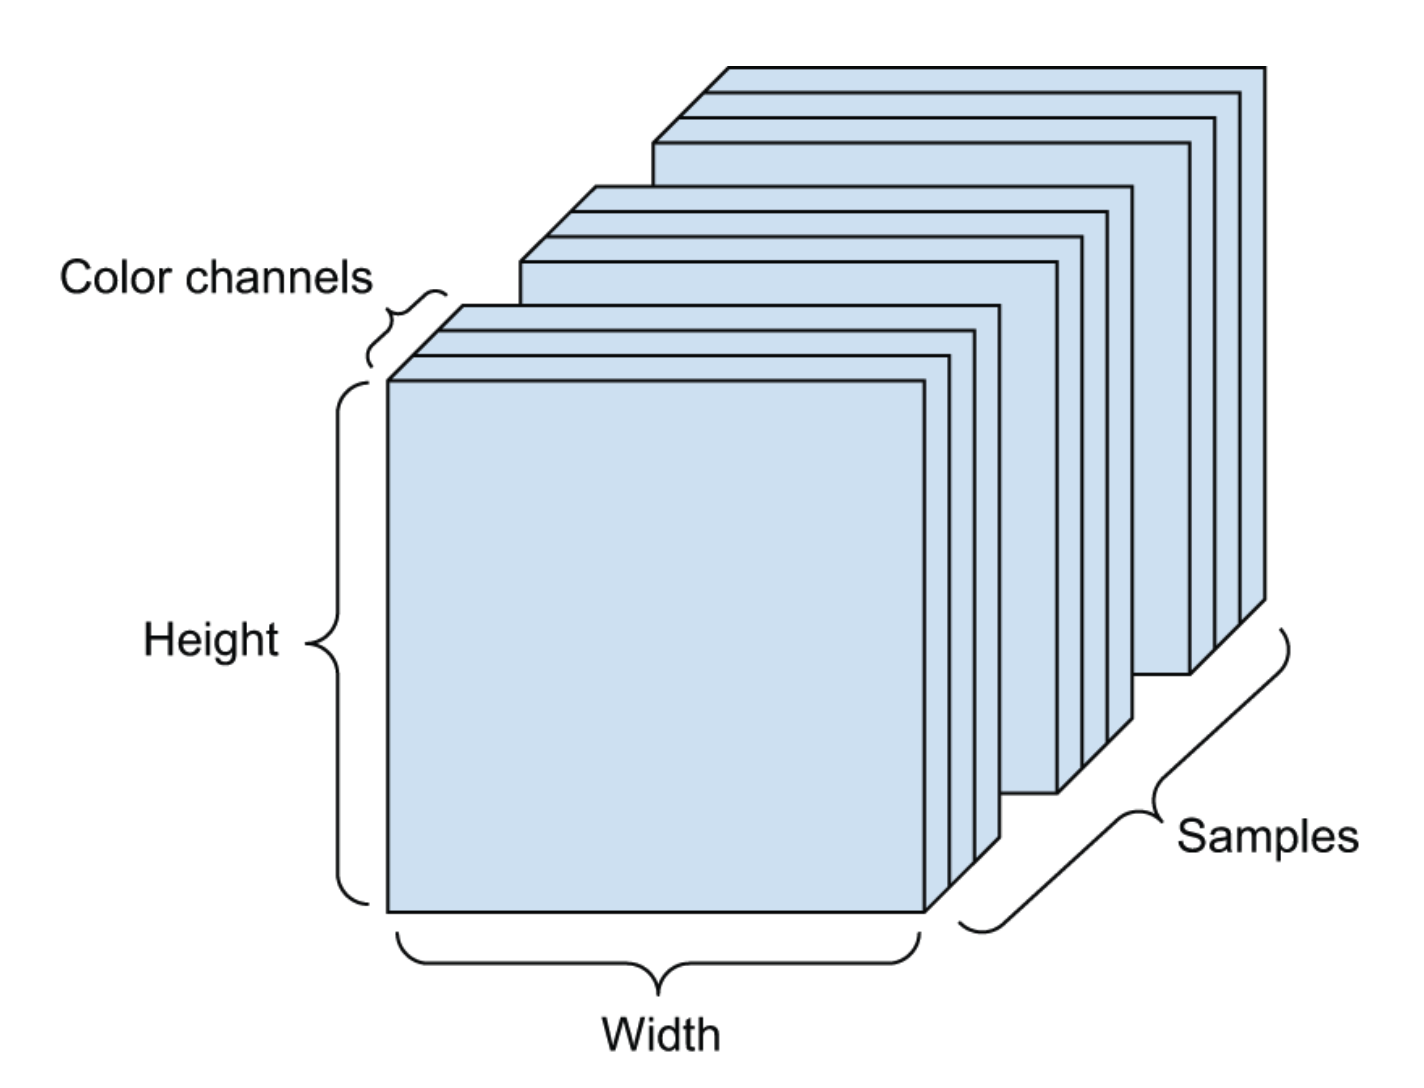
\includegraphics[scale=.3]{img/1.png}
\end{frame}

\begin{frame}{Tensor Operations}
    \begin{itemize}
        \item Just like programs reduce to simple binary operations (AND, OR, NOR),
              deep learning reduces to a small set of \textit{tensor operations}.

        \item These operations (or \textit{tensor functions}) are applied to numerical data.

        \item Common examples:
              \begin{itemize}
                  \item Addition
                  \item Multiplication
                  \item Other element-wise transformations
              \end{itemize}
    \end{itemize}
\end{frame}

\begin{frame}[fragile]{Element-wise Operations}
    \begin{itemize}
        \item Element-wise operations are applied independently to each entry of a tensor.
        \item Examples: addition, ReLU (\texttt{max(x, 0)}).
        \item These operations are highly parallelizable (vectorized).
    \end{itemize}

    \begin{center}
        \begin{tcolorbox}[
                width=0.75\textwidth,
                colback=gray!5,
                colframe=gray!60,
                boxrule=0.4pt,
                arc=3pt,
                left=6pt,right=6pt,top=6pt,bottom=6pt
            ]
            \begin{minted}{python}
def naive_relu(x):
    x = x.copy()
    for i in range(x.shape[0]):
        for j in range(x.shape[1]):
            x[i, j] = max(x[i, j], 0)
    return x
\end{minted}
        \end{tcolorbox}
    \end{center}

    \vspace{0.5em}
    \small In practice, this is done without loops using vectorized operations.
\end{frame}

\begin{frame}[fragile]{Element-wise Addition}
    \begin{itemize}
        \item Addition can also be applied element-wise to tensors.
        \item Both tensors must have the same shape.
        \item Like ReLU, this operation is naturally parallelizable.
    \end{itemize}

    \begin{center}
        \begin{tcolorbox}[
                width=0.75\textwidth,
                colback=gray!5,
                colframe=gray!60,
                boxrule=0.4pt,
                arc=3pt,
                left=6pt,right=6pt,top=6pt,bottom=6pt
            ]
            \begin{minted}{python}
def naive_add(x, y):
    x = x.copy()
    for i in range(x.shape[0]):
        for j in range(x.shape[1]):
            x[i, j] += y[i, j]
    return x
\end{minted}
        \end{tcolorbox}
    \end{center}

    \vspace{0.5em}
    \small In practice: \texttt{x + y} (vectorized, no loops needed).
\end{frame}

\begin{frame}[fragile]{Broadcasting}
    \begin{itemize}
        \item Broadcasting allows operations on tensors with different shapes.
        \item The smaller tensor is automatically expanded to match the larger one.
    \end{itemize}

    \vspace{0.3em}
    \textbf{How it works:}
    \begin{itemize}
        \item Add missing axes to the smaller tensor
        \item Repeat values along those axes to match the shape
    \end{itemize}

    \begin{center}
        \begin{tcolorbox}[
                width=0.75\textwidth,
                colback=gray!5,
                colframe=gray!60,
                boxrule=0.4pt,
                arc=3pt,
                left=6pt,right=6pt,top=6pt,bottom=6pt
            ]
            \begin{minted}{python}
import numpy as np

x = np.random.random((32, 10))  # matrix
y = np.random.random((10,))     # vector

z = x + y  # broadcasting
\end{minted}
        \end{tcolorbox}
    \end{center}

    \vspace{0.5em}
    \small Example: (32, 10) + (10,) → (32, 10)
\end{frame}

\begin{frame}[fragile]{Broadcasting (Implementation Insight)}
    \begin{itemize}
        \item Broadcasting does \textbf{not} actually copy data in memory.
        \item The expansion is \textit{virtual} (done at the algorithm level).
        \item Still, it’s useful to think of the smaller tensor as being repeated.
    \end{itemize}

    \begin{center}
        \begin{tcolorbox}[
                width=0.75\textwidth,
                colback=gray!5,
                colframe=gray!60,
                boxrule=0.4pt,
                arc=3pt,
                left=6pt,right=6pt,top=6pt,bottom=6pt
            ]
            \begin{minted}{python}
def naive_add_matrix_and_vector(x, y):
    x = x.copy()
    for i in range(x.shape[0]):
        for j in range(x.shape[1]):
            x[i, j] += y[j]
    return x
\end{minted}
        \end{tcolorbox}
    \end{center}

    \vspace{0.5em}
    \small In practice: \texttt{x + y} uses broadcasting (no loops, no copies).
\end{frame}

\begin{frame}[fragile]{Tensor Product (Dot Product)}
    \begin{itemize}
        \item The \textit{tensor product} (dot product / matmul) is a fundamental operation.
        \item It combines tensors through multiplication and summation.
    \end{itemize}

    \begin{center}
        \begin{tcolorbox}[
                width=0.75\textwidth,
                colback=gray!5,
                colframe=gray!60,
                boxrule=0.4pt,
                arc=3pt,
                left=6pt,right=6pt,top=6pt,bottom=6pt
            ]
            \begin{minted}{python}
import numpy as np

x = np.random.random((32,))
y = np.random.random((32,))

z = np.matmul(x, y)
# equivalent:
z = x @ y
\end{minted}
        \end{tcolorbox}
    \end{center}

    \vspace{0.5em}
    \small Mathematical notation: $z = x \cdot y$
\end{frame}

\begin{frame}[fragile]{Dot Product (Vector $\times$ Vector)}
    \begin{itemize}
        \item The dot product multiplies two vectors and sums the results.
        \item The result is a \textit{scalar}.
        \item Vectors must have the same length.
    \end{itemize}

    \begin{center}
        \begin{tcolorbox}[
                width=0.75\textwidth,
                colback=gray!5,
                colframe=gray!60,
                boxrule=0.4pt,
                arc=3pt,
                left=6pt,right=6pt,top=6pt,bottom=6pt
            ]
            \begin{minted}{python}
def naive_vector_product(x, y):
    z = 0.0
    for i in range(x.shape[0]):
        z += x[i] * y[i]
    return z
\end{minted}
        \end{tcolorbox}
    \end{center}

    \vspace{0.5em}
    \small Mathematical form: $z = \sum_i x_i y_i$
\end{frame}

\begin{frame}[fragile]{Matrix $\times$ Vector Product}
    \begin{itemize}
        \item Multiplying a matrix $X$ by a vector $y$ returns a vector.
        \item Each output element is the dot product of a row of $X$ with $y$.
    \end{itemize}

    \begin{center}
        \begin{tcolorbox}[
                width=0.78\textwidth,
                colback=gray!5,
                colframe=gray!60,
                boxrule=0.4pt,
                arc=3pt,
                left=6pt,right=6pt,top=6pt,bottom=6pt
            ]
            \begin{minted}{python}
def naive_matrix_vector_product(x, y):
    z = np.zeros(x.shape[0])
    for i in range(x.shape[0]):
        for j in range(x.shape[1]):
            z[i] += x[i, j] * y[j]
    return z
\end{minted}
        \end{tcolorbox}
    \end{center}

    \vspace{0.5em}
    \small Equivalent view:
    \texttt{z[i] = dot(x[i, :], y)}

    \vspace{0.3em}
    \small Not symmetric: \texttt{matmul(x, y) $\neq$ matmul(y, x)}
\end{frame}

\begin{frame}{A schematic representation of tensor products}
    \centering
    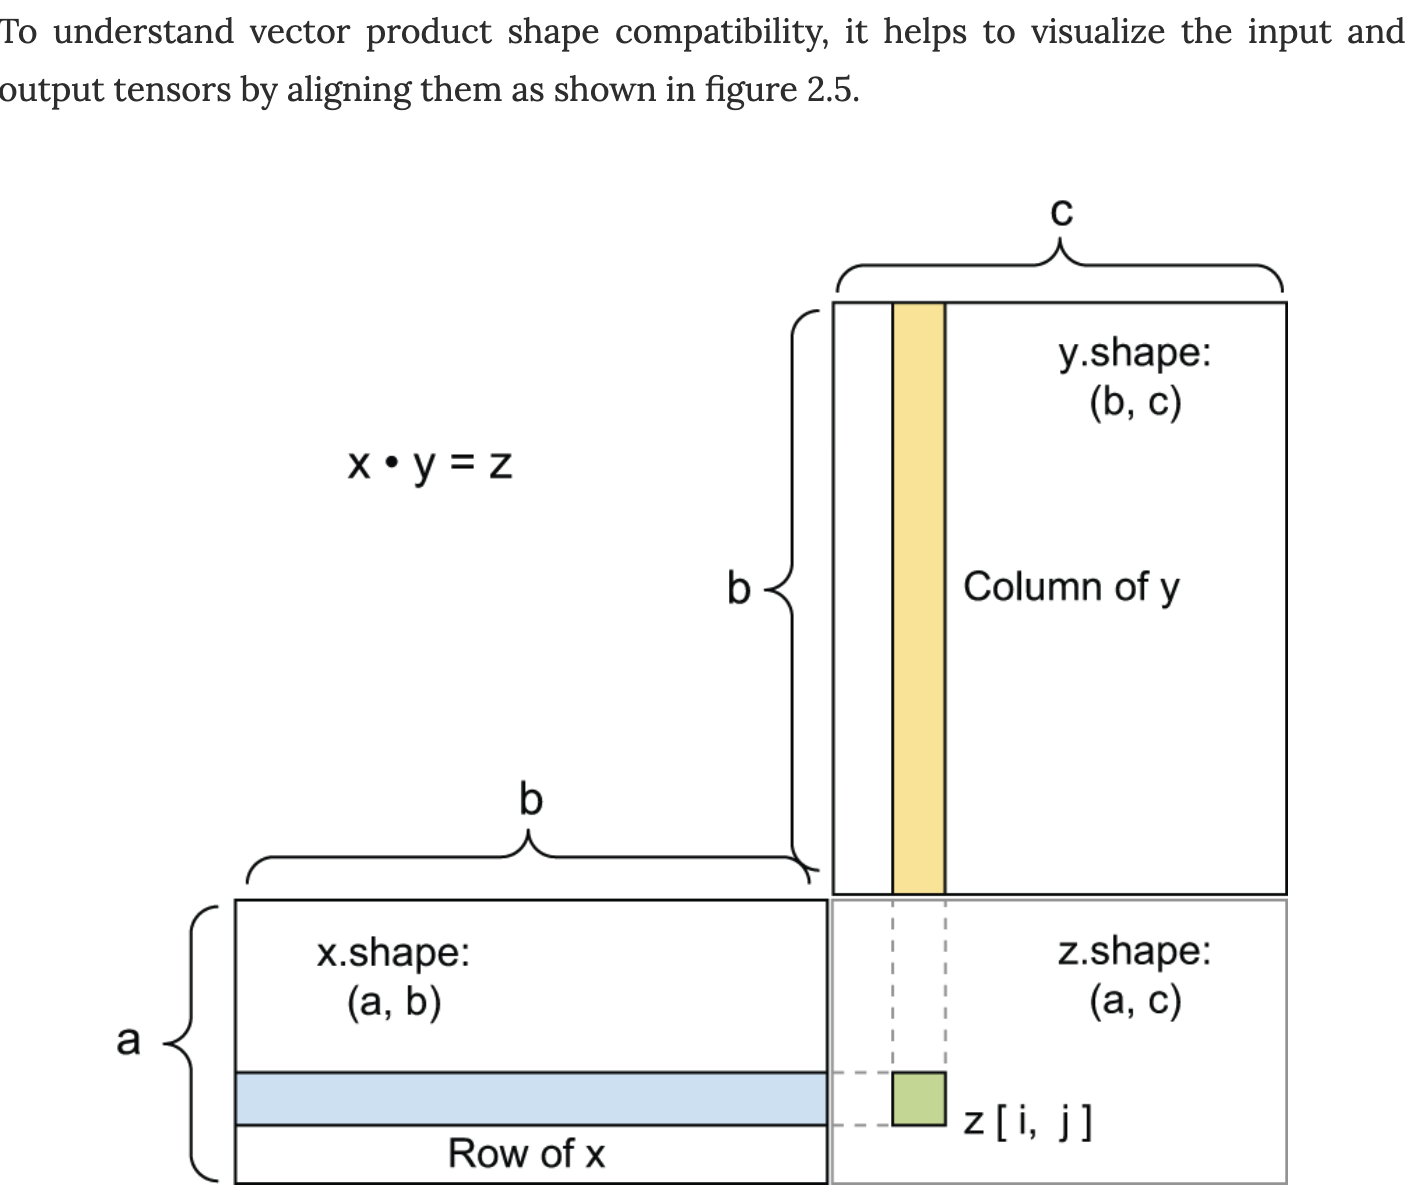
\includegraphics[scale=.3,trim=0 0 0 2cm, clip]{img/2.png}
\end{frame}

\begin{frame}[fragile]{Tensor Reshaping}
    \begin{itemize}
        \item Reshaping changes the shape of a tensor without changing its data.
        \item The total number of elements must remain the same.
    \end{itemize}

    \begin{center}
        \begin{tcolorbox}[
                width=0.78\textwidth,
                colback=gray!5,
                colframe=gray!60,
                boxrule=0.4pt,
                arc=3pt,
                left=6pt,right=6pt,top=6pt,bottom=6pt
            ]
            \begin{minted}{python}
import numpy as np

x = np.array([[0, 1],
              [2, 3],
              [4, 5]])   # shape (3, 2)

x = x.reshape((6, 1))
# shape (6, 1)

x = x.reshape((2, 3))
# shape (2, 3)
\end{minted}
        \end{tcolorbox}
    \end{center}

    \vspace{0.5em}
    \small Same data, different shapes.
\end{frame}

\begin{frame}{The Engine of Neural Networks}
    \begin{itemize}
        \item Each layer transforms input as:
    \end{itemize}

    \vspace{0.5em}
    \centering
    \texttt{output = relu(matmul(input, W) + b)}

    \vspace{0.5em}
    \begin{itemize}
        \item $W$, $b$ are \textit{trainable parameters} (weights and bias)
        \item Initially random → produce meaningless outputs
        \item Learning = adjusting these parameters
    \end{itemize}
\end{frame}

\begin{frame}{How Training Works}
    \begin{itemize}
        \item Sample a batch: $x$, $y_{\text{true}}$
        \item Compute predictions: $y_{\text{pred}}$
        \item Compute loss (error)
        \item Update weights to reduce loss
    \end{itemize}

    \vspace{0.5em}
    \small Goal: minimize difference between $y_{\text{pred}}$ and $y_{\text{true}}$
\end{frame}

\begin{frame}{Why Not Try All Values?}
    \begin{itemize}
        \item Idea: tweak one weight, check if loss improves
        \item Repeat for all weights
    \end{itemize}

    \vspace{0.5em}
    \begin{itemize}
        \item Works in theory…
        \item But extremely slow (millions/billions of parameters)
    \end{itemize}

    \vspace{0.5em}
    \centering
    \textit{We need a smarter way → Gradient Descent}
\end{frame}

\begin{frame}{Gradient Descent Intuition}
    \begin{itemize}
        \item Model functions are \textit{smooth} (differentiable)
        \item Small change in weights → small change in loss
        \item Gradient tells us:
              \begin{itemize}
                  \item Which direction reduces the loss
                  \item How much to adjust
              \end{itemize}
    \end{itemize}

    \vspace{0.5em}
    \centering
    \textit{Update all weights at once in the right direction}
\end{frame}

\begin{frame}{What’s a Derivative?}
    \begin{itemize}
        \item A function maps input to output: $f(x) = y$
        \item The derivative measures:
              \begin{itemize}
                  \item How much $y$ changes when $x$ changes
              \end{itemize}
    \end{itemize}

    \vspace{0.5em}
    \centering
    \textit{Derivative = slope = rate of change}
\end{frame}

\begin{frame}{Gradient Descent: visual intuition}
    \centering
    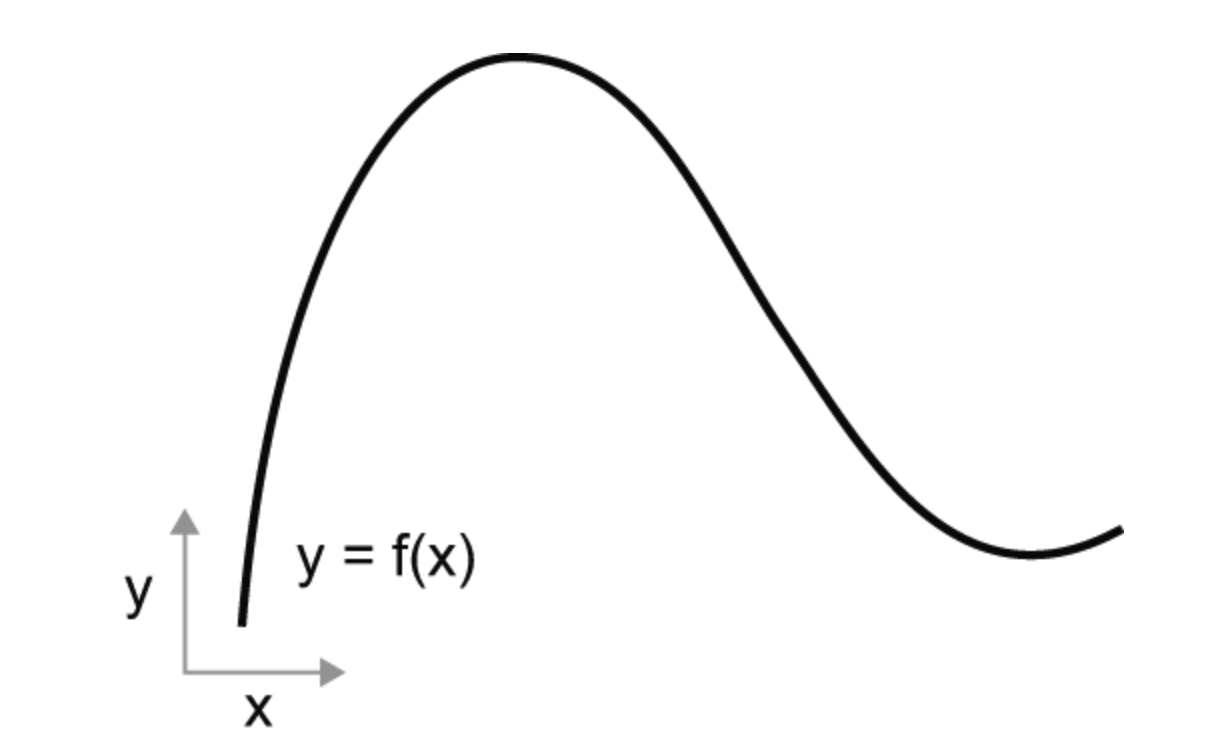
\includegraphics[scale=.3]{img/3.png}
\end{frame}

\begin{frame}{Gradient Descent: visual intuition}
    \centering
    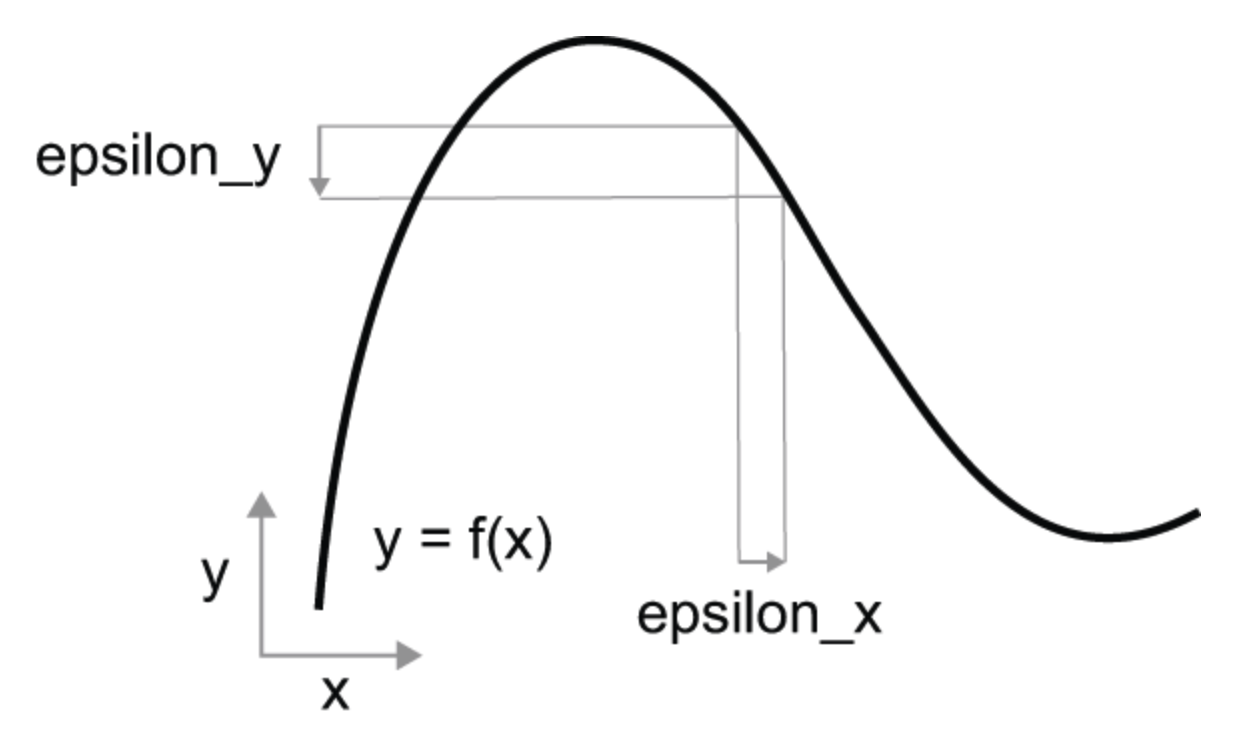
\includegraphics[scale=.3]{img/4.png}
\end{frame}

\begin{frame}{Gradient Descent: visual intuition}
    \centering
    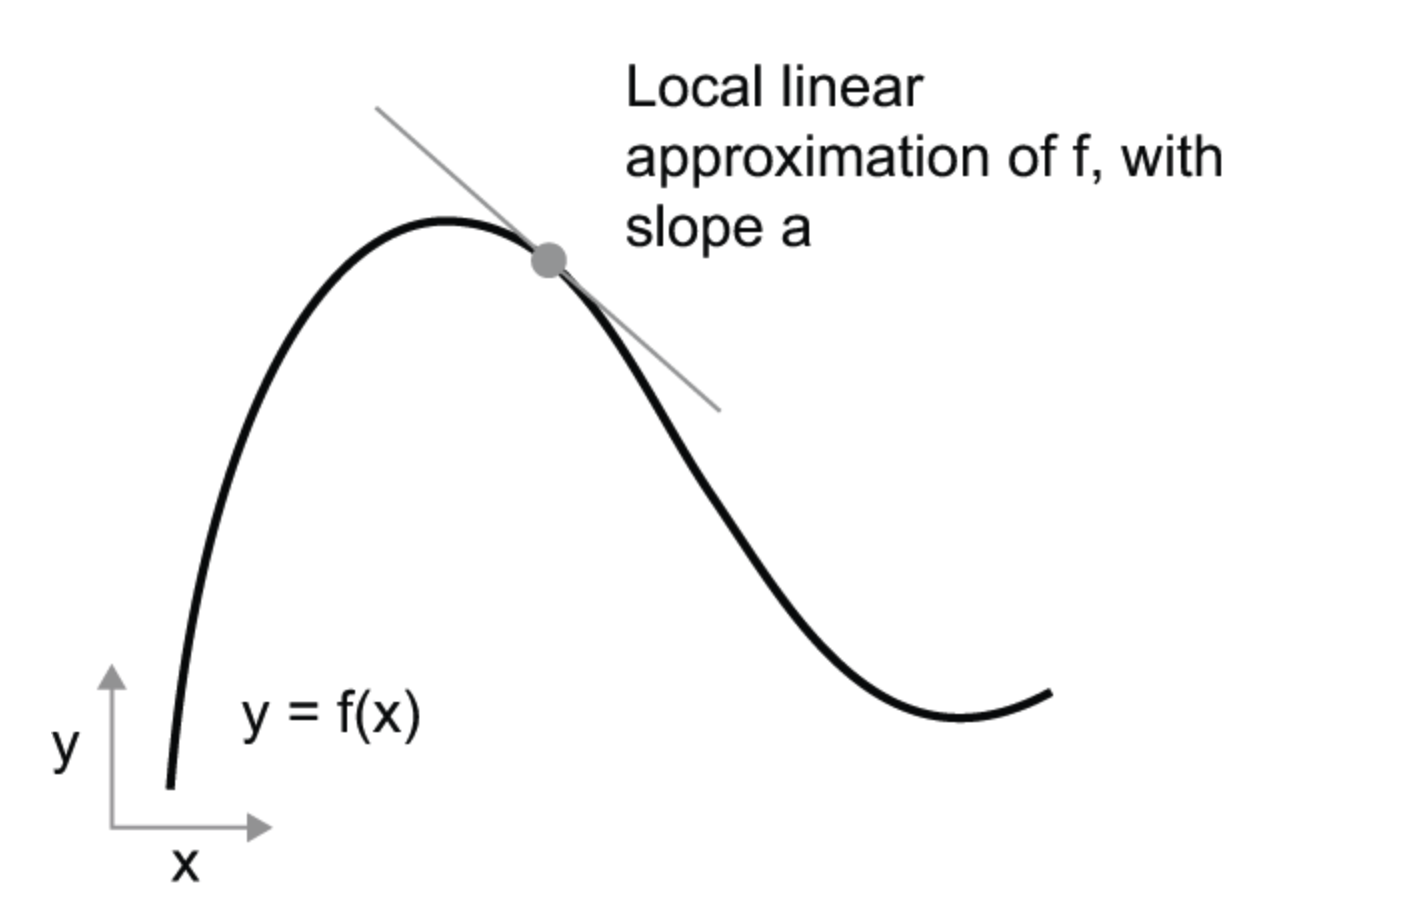
\includegraphics[scale=.3]{img/5.png}
\end{frame}

\begin{frame}{Gradient: Derivative of Tensor Functions}
    \begin{itemize}
        \item A function can map:
              \begin{itemize}
                  \item Scalar $\to$ scalar → curve
                  \item Vector $\to$ scalar → surface
                  \item Tensor $\to$ scalar → higher-dimensional surface
              \end{itemize}

        \item The \textit{gradient} is the generalization of the derivative.
        \item It tells us how the output changes when inputs change.
    \end{itemize}

    \vspace{0.5em}
    \centering
    \textit{Derivative = slope (1D)} \\
    \textit{Gradient = direction of steepest change (multi-D)}
\end{frame}

\begin{frame}{Stochastic Gradient Descent (SGD)}
    \begin{itemize}
        \item In theory: find minimum by solving $\nabla f(W) = 0$
        \item In practice: impossible for large models (millions of parameters)
    \end{itemize}

    \vspace{0.5em}
    \begin{itemize}
        \item Instead: iteratively update parameters using gradients
        \item Move weights in the direction that reduces the loss
    \end{itemize}

    \vspace{0.5em}
    \centering
    \texttt{W = W - learning\_rate * gradient}
\end{frame}

\begin{frame}{SGD Algorithm (Mini-batch)}
    \begin{itemize}
        \item Sample a batch: $x$, $y_{\text{true}}$
        \item Forward pass → compute $y_{\text{pred}}$
        \item Compute loss
        \item Backward pass → compute gradient
        \item Update weights
    \end{itemize}

    \vspace{0.5em}
    \small learning\_rate controls step size
\end{frame}

\begin{frame}{Key Ideas Behind SGD}
    \begin{itemize}
        \item Uses random batches (stochastic = random)
        \item Efficient for large datasets
        \item Updates happen step-by-step (not all at once)
    \end{itemize}

    \vspace{0.5em}
    \centering
    \textit{Gradually reduces loss over time}
\end{frame}

\begin{frame}{Stochastic Gradient Descent (SGD) Intuition}
    \centering
    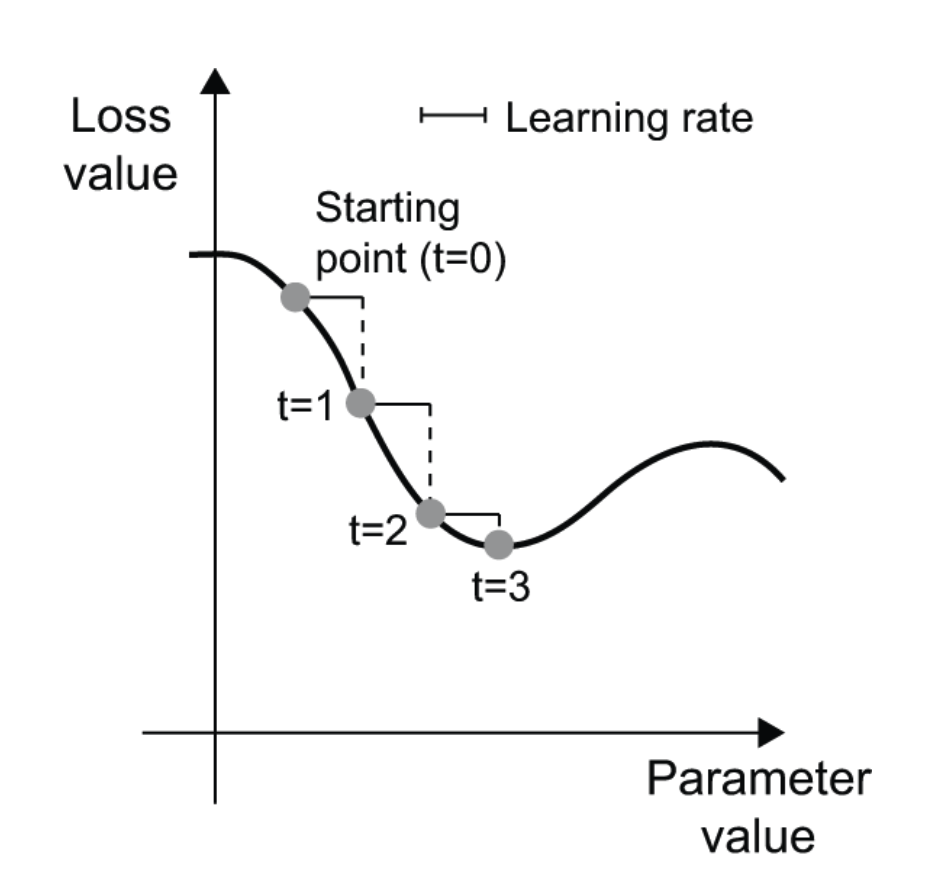
\includegraphics[scale=.3]{img/6.png}
\end{frame}

\begin{frame}{Stochastic Gradient Descent (SGD) Intuition}
    \centering
    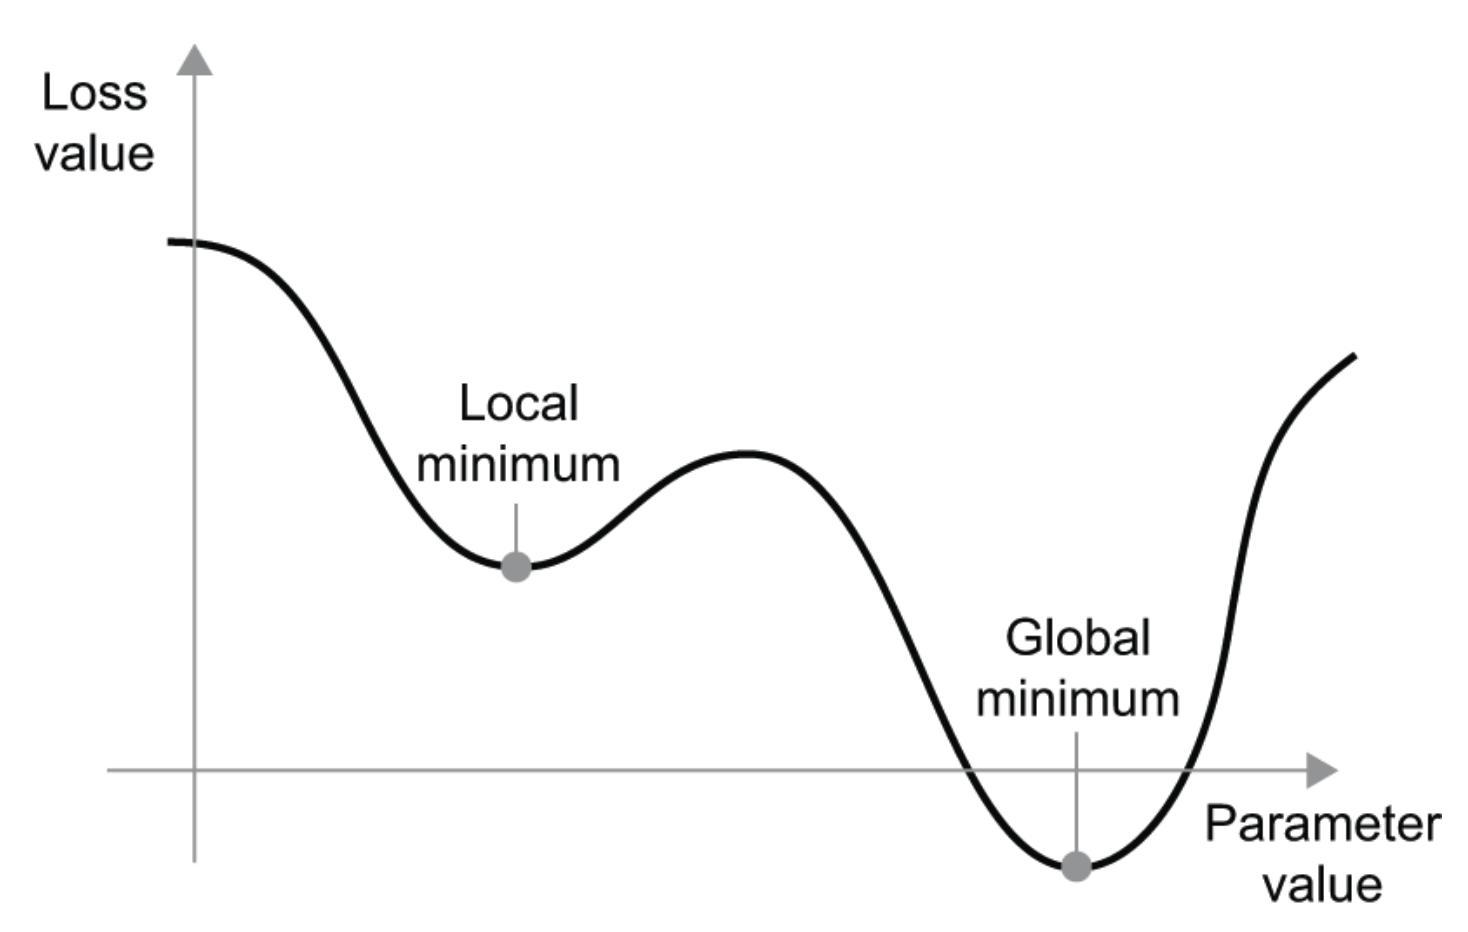
\includegraphics[scale=.3]{img/7.png}
\end{frame}

% \begin{frame}{How Learning (Backpropagation) Works}
    \centering
    \animategraphics[
        controls,
        loop,
        poster=first,
        width=.86\paperwidth
    ]{3}{backprop_frames/backprop-}{000}{069}
\end{frame}
\end{document}